\documentclass[border=6pt]{standalone}
\usepackage{amsmath,tikz}
\usetikzlibrary{arrows.meta,calc,positioning}
\begin{document}
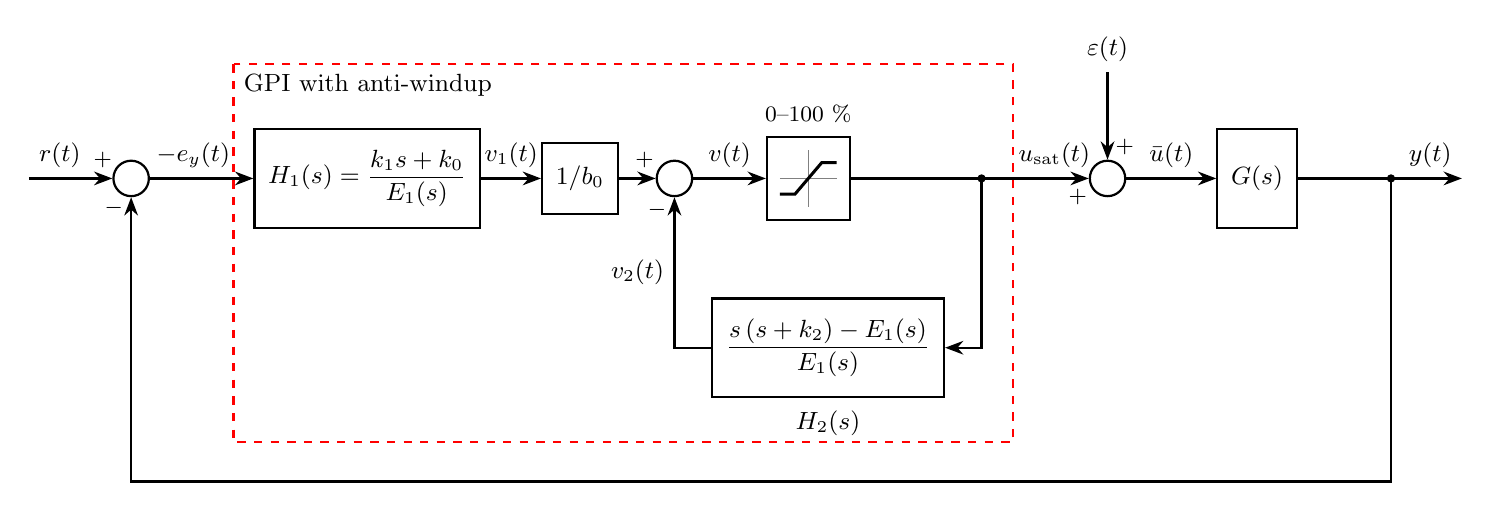
\begin{tikzpicture}[>=Stealth, thick, font=\small,
  block/.style={draw, thick, fill=white, align=center, minimum height=1.25cm, inner sep=5pt},
  sum/.style={draw, thick, circle, minimum size=0.45cm, inner sep=0pt},
  sgn/.style={font=\footnotesize, inner sep=0pt}]
  \node[sum] (s1) at (0.9,0) {};
  \node[block] (h1) at (3.9,0) {$H_1(s) = \dfrac{k_1 s + k_0}{E_1(s)}$};
  \node[block, minimum height=0.9cm] (ib) at (6.6,0) {$1/b_0$};
  \node[sum] (s2) at (7.8,0) {};
  \node[block, minimum size=1.05cm] (sat) at (9.5,0) {};
  \draw[thin, gray] ($(sat.center)+(-0.36,0)$) -- ($(sat.center)+(0.36,0)$);
  \draw[thin, gray] ($(sat.center)+(0,-0.36)$) -- ($(sat.center)+(0,0.36)$);
  \draw[line width=1.1pt] ($(sat.center)+(-0.36,-0.2)$) -- ($(sat.center)+(-0.17,-0.2)$)
     -- ($(sat.center)+(0.17,0.2)$) -- ($(sat.center)+(0.36,0.2)$);
  \node[above=1pt of sat, font=\footnotesize] {0--100 \%};
  \coordinate (us) at (11.7,0);
  \node[block] (h2) at (9.75,-2.15) {$\dfrac{s\,(s + k_2) - E_1(s)}{E_1(s)}$};
  \node[below=1pt of h2] {$H_2(s)$};
  \node[sum] (s3) at (13.3,0) {};
  \node[block] (g) at (15.2,0) {$G(s)$};
  \coordinate (yb) at (16.9,0);
  \draw[red, dashed] (2.2,1.45) rectangle (12.1,-3.35);
  \node[below right, font=\small] at (2.2,1.45) {GPI with anti-windup};
  \draw[->] (-0.4,0) node[above right] {$r(t)$} -- (s1.west);
  \node[sgn] at ($(s1.west)+(-0.12,0.24)$) {$+$};
  \draw[->] (s1.east) -- node[above, pos=0.42] {$-e_y(t)$} (h1.west);
  \draw[->] (h1.east) -- node[above] {$v_1(t)$} (ib.west);
  \draw[->] (ib.east) -- (s2.west);
  \node[sgn] at ($(s2.west)+(-0.14,0.24)$) {$+$};
  \draw[->] (s2.east) -- node[above] {$v(t)$} (sat.west);
  \draw (sat.east) -- (us); \fill (us) circle (1.5pt);
  \draw[->] (us) -- node[above, pos=0.68] {$u_{\mathrm{sat}}(t)$} (s3.west);
  \node[sgn] at ($(s3.west)+(-0.14,-0.24)$) {$+$};
  \draw[->] (13.3,1.35) node[above] {$\varepsilon(t)$} -- (s3.north);
  \node[sgn] at ($(s3.north)+(0.22,0.16)$) {$+$};
  \draw[->] (s3.east) -- node[above] {$\bar u(t)$} (g.west);
  \draw[->] (us) -- (us |- h2) -- (h2.east);
  \draw[->] (h2.west) -- (s2 |- h2) -- node[left, pos=0.5] {$v_2(t)$} (s2.south);
  \node[sgn] at ($(s2.south)+(-0.22,-0.16)$) {$-$};
  \draw (g.east) -- (yb); \fill (yb) circle (1.5pt);
  \draw[->] (yb) -- (17.8,0) node[above left] {$y(t)$};
  \draw[->] (yb) -- (16.9,-3.85) -- (0.9,-3.85) -- (s1.south);
  \node[sgn] at ($(s1.south)+(-0.22,-0.14)$) {$-$};
\end{tikzpicture}
\end{document}
